\section{Panoramica del sito}
All'apertura del sito, l'utente visualizza immediatamente una lista di dataset selezionabili di vario genere.
\begin{figure}[h!]
    \centering
    
\includegraphics[scale=0.6]{template/images/placeholder.png}
    \caption{Schermata di selezione dataset}
\end{figure}
\newline
\newline
L'utente può espandere ciascun elemento della lista per accedere a una vista dettagliata con maggiori informazioni.
\begin{figure}[h!]
    \centering
    
\includegraphics[scale=0.6]{template/images/placeholder.png}
    \caption{Maggiori dettagli}
\end{figure}
\newline
\newline
Dopo aver selezionato un dataset, l'utente dovrà attendere il caricamento dei dati. Al termine, verrà reindirizzato all'ambiente 3D.
\begin{figure}[h!]
    \centering
    
\includegraphics[scale=0.6]{template/images/placeholder.png}
    \caption{Ambiente 3D}
\end{figure}
\newpage


\subsection{Funzionalità}
Una volta entrato con successo nell'ambiente 3D l'utente può eseguire operazioni come:
\begin{itemize}
    \item Hover del mouse sulle barre del grafico per mostrare attraverso un tooltip che valore viene rappresentato;
    \item Spostamento e zoom della vista;
    \item Rotazione del grafico;
    \item Reset della visuale;
    \item Interazione con i dati in forma tabellare;
    \item Filtraggio dei valori superiori o inferiori al valor medio;
    \item Filtraggio dei valori superiori o inferiori rispetto ad un dato valore imposto dall'utente;
    \item Filtrare gli N valori più bassi o più alti.
\end{itemize}

\section{Interfaccia utente}

\section{Navigazione}
All’interno dell'ambiente 3D l'utente può interagire con la vista attraverso l'utilizzo del mouse:
\begin{itemize}
    \item \textbf{Spostamento:} spostando il cursore del mouse tenendo premuto il tasto sinistro;
    \item \textbf{Zoom-in/out:} rotella del mouse;
    \item \textbf{Rotazione:} spostando il cursore del mouse tenendo premuto il tasto destro;
    \item \textbf{Reset visuale:} premendo il tasto "R" della tastiera vista viene riportata alla posizione iniziale;
\end{itemize}
\clearpage
\begin{figure}[ht!]
    \centering
    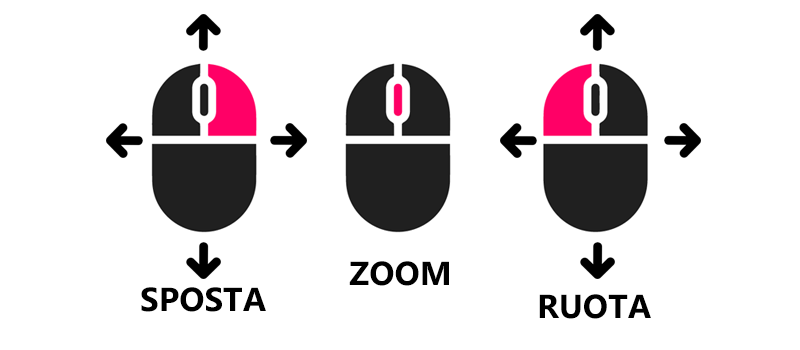
\includegraphics[scale=0.6]{template/images/comandi.png}
    \caption{Comandi per la navigazione}
\end{figure}


